\chapter{Die Analyse und Tests}
\label{cha:Analyse}
Dieses Kapitel beschäftigt sich mit der Analyse der Implementierung und dessen Tests. Es gibt zwei Arten von Tests die implementiert wurden
\begin{itemize}
	\item die \emph{JUnit}-Tests sind die Tests, die nicht auf eine \emph{CDI}-Umgebung angewiesen sind und 
	\item die \emph{CDI-JUnit}-Tests sind die Tests, die auf eine \emph{CDI}-Umgebung angewiesen sind.
\end{itemize}

\section{Die Tests}
Dieser Abschnitt beschäftigt sich mit den Implementieren Tests des Vorlagenmanagements und der Implementierten Konfiguration für die Tests. Für die Tests wurden folgende Bibliotheken verwendet.
\begin{itemize}
	\item\emph{JUnit4} ist ein \emph{Framework}, mit dem wiederholbare Tests implementiert werden können und ist als Standard für Tests in \emph{Java} anzusehen.
	\item\emph{Deltaspike} ist ein \emph{Open-Source}-Projekt der \emph{Apache Software Foundation (ASF)}, die portable \emph{CDI}-Erweiterungen in Form von Modulen bereitstellt und auch eine Erweiterung für \emph{JUnit}-Tests bereitstellt, mit denen Tests in einer \emph{CDI}-Umgebung lauffähig sind.
\end{itemize}
\ \newline
Alle implementierten Tests sind nicht auf einen Anwendungsserver angewiesen und sind innerhalb des lokalen Klassenpfades lauffähig und können daher in jeder Entwicklungsumgebung und bei einem Kompilieren über das \emph{Buildtool Maven} ausführbar.
\newline
\newline
Die Tests wurden wie folgt organisiert.
\begin{itemize}
	\item\emph{com.clevercure.mailing.test.*} 
	\newline
	ist das \emph{Java}-Paket in dem alle implementierten Tests liegen. 
	\item\emph{*.[toTestClass]Tests}
	\newline
	ist das \emph{Java}-Paket, für eine zu testende Klasse, wobei der Paketname den Namen der zu testenden Klasse mit dem Suffix Tests enthält.
	\item\emph{[toTestMethod]Test.java}
	\newline
	ist die implementierte Testklasse für die Tests einer Methode der zu testenden Klasse.
	\item\emph{test\_case}
	\newline
	ist der Name der einzelnen Testmethoden, der wiedergibt was an einer Methode getestet wird. 
\end{itemize}
\ \newline
Die vorgestellte Konvention der Tests wurde so umgesetzt sofern es möglich war. 

\subsection{Die Tests der \emph{CDI}-Erweiterung}
Die Tests aus Abbildung \ref{fig:tests-template-cdi} testen die Implementierungen des Artefakts \emph{mailing-moule-template-cdi} wie
\begin{itemize}
	\item die Klasse \emph{TemplateCdiExtension},
	\item die Klasse \emph{CdiTemplateUtils} und
	\item die Klasse \emph{TemplateResourceProducer}.
\end{itemize}
\begin{figure}[h]
\centering
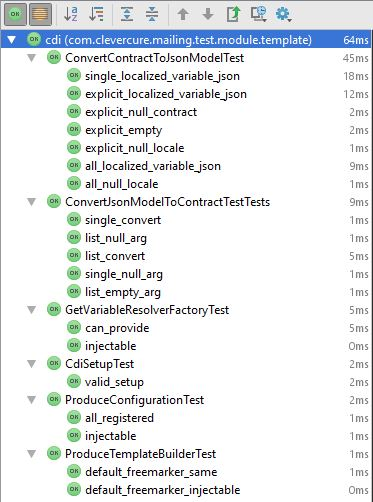
\includegraphics[scale=0.8]{tests-template-cdi}
\caption{Testdurchlauf der Tests der \emph{CDI}-Erweiterung}
\label{fig:tests-template-cdi}
\end{figure}
\ \newline
Diese Tests sind nur lauffähig in einer \emph{CDI}-Umgebung, die aber Dank \emph{Deltaspike} auch im Klassenpfad ohne Anwendungsserver gestartet werden kann. Im Klassenpfad der Tests wurde Variablen über eine \emph{Enumeration}, die die Schnittstelle \emph{VariableContract} implementiert, definiert, sowie eine Implementierung der Klasse \emph{VariableResolverFactory}.

\subsection{Die Tests des Vorlagenmanagements}
Die Tests aus Abbildung \ref{fig:tests-template-cdi} testen die Implementierungen des Artefakts \emph{mailing-moule-template-logic-impl} wie
\begin{itemize}
	\item die Klasse \emph{VariableConfigurationImpl} und
	\item die Klasse \emph{FreemarkerTemplateDataJsonBuilder}.
\end{itemize}
\ \newline
\emph{TODO: Add image of running tests}
\newline
Diese Tests sind nicht angewiesen auf eine \emph{CDI}-Umgebung und sind ohne zusätzliche Bibliotheken und \emph{Framwork} lauffähig. Sie Testen die implementierten Methoden und vor allem bezüglich derer Fehlerbehandlung.

\section{Die erreichten Ziele}
Dieser Abschnitt beschäftigt sich mit der Betrachtung der erreichten Ziele des Vorlagenmanagements. Es wurden alle Anforderung aus dem Kapitel \ref{cha:Zielsetzung} erfüllt, somit gilt das Vorlagenmanagement als abgeschlossen. Die Integrationen in die Anwendungen \emph{CleverWeb} und \emph{CleverInterface} wurde noch nicht realisiert, obwohl begonnen wurde eine Integration für die Anwendung in \emph{CleverWeb} zu implementieren. Die Integration in die Anwendung \emph{CleverInterface} wird erst realisiert werden können, wenn diese Anwendung \emph{Java} in Version 8 unterstützt. Zurzeit wird nur \emph{Java} in version 7 unterstützt. 

\subsection{Das Vorlagenmanagement \emph{CKEditor-Plugin}}
Es wurde erfolgreich ein \emph{Plugin} in \emph{Typescript} für den \emph{CKEditor} implementiert, dass das Variablenmanagement erfolgreich in diesen \emph{Editor} integriert. Dies war vor allem möglich, da von \emph{DefinitelyType} Typinformationen zur Verfügung gestellt werden, obwohl diese ein paar Fehler beinhalteten, die aber leicht ausgebessert wurden. Die implementierten Typescrript Quelltexte befinden sich zurzeit noch in der Demowebanwendung, da die Entwicklung in einem eigenen Projekt nicht möglich war, da das \emph{Hot-Code-Deployment} für \emph{Java}-Ressourcen (src/main/resources) nicht unterstützt wird. Diese Quelltextdateien, können aber einfach verschoben werden. Die Entwicklung des 

\subsection{Das Vorlagen-\emph{Management} in einer \emph{CDI}-Umgebung}

\subsection{Das Vorlagen-\emph{Management} in JSF}
\subsection{Das Vorlagen-\emph{Management} in \emph{Mail}-DB-Schema}

